\documentclass[../../main-ap-physics.tex]{subfiles}

\begin{document}

\section{Dynamics: Force and Newton's Laws of Motion}

\subsection{Development of Force Concept}

\Gls{dynamics} is the study of the forces that cause objects and systems to move. To understand this, we need a working definition of \gls{force}. Our intuitive definition of force---that is, a push or a pull---is a good place to start. We know that a push or pull has both magnitude and direction (therefore, it is a vector quantity) and can vary considerably in each regard. For example, a cannon exerts a strong force on a cannonball that is launched into the air. In contrast, Earth exerts only a tiny downward pull on a flea. Our everyday experiences also give us a good idea of how multiple forces add. If two people push in different directions on a third person, as illustrated in Figure \ref{KPYGZu}, we might expect the total force to be in the direction shown. Since force is a vector, it adds just like other vectors, as illustrated in Figure \ref{KPYGZu}(a) for two ice skaters. Forces, like other vectors, are represented by arrows and can be added using the familiar head-to-tail method or by trigonometric methods. These ideas were developed in ``Two-Dimensional Kinematics.''

\begin{center}
    \begin{tikzpicture}
        \begin{axis}[width=6cm,
            xmin=0,xmax=10,
            ymin=0,ymax=10,
            ticks=none,
            axis line style={draw=none},
            clip=false,
        ]
        \draw[->,red,thick] (0,5) node[below,black] {$F_1$} -- ++(5,0);
        \draw[->,red,thick] (5,0) node[left,black] {$F_2$} -- ++(0,5);
        \begin{scope}[shift={(5.25,0.25)}]
            \draw[->,red,dashed] (0,5) -- ++(5,0) node[below,pos=0.5,black] {$F_1$};
            \draw[->,red,dashed] (5,5) -- ++(0,5) node[right,pos=0.5,black] {$F_2$};
            \draw[->,red,thick] (0,5) -- ++(5,5) node[above left,pos=0.5,black] {$F_{\text{tot}}$};
        \end{scope}
        \node at (1,9) {(a)};
        \end{axis}
    \end{tikzpicture}%
    \hspace{1cm}
    \begin{tikzpicture}
        \begin{axis}[width=6cm,
            xmin=0,xmax=10,
            ymin=0,ymax=10,
            ticks=none,
            axis line style={draw=none},
            clip=false,
        ]
        \draw[->,thick] (5pt,0) -- ++(5,0) node[below,pos=0.5] {$F_1$};
        \draw[->,thick] (0,5pt) -- ++(0,5) node[left,pos=0.5] {$F_2$};
        \fill[red] (0,0) circle (3pt);
        \node[right] at (1,6) {Free-body diagram};
        \node at (1,8) {(b)};
        \end{axis}
    \end{tikzpicture}
    \captionsetup{type=figure,margin=1in,font=scriptsize}
    \captionof{figure}{Part (a) shows an overhead view of two ice skaters pushing on a third. Forces are vectors and add like other vectors, so the total force on the third skater is in the direction shown. In part (b), we see a free-body diagram representing the forces acting on the third skater.}
    \label{KPYGZu}
\end{center}

Figure \ref{KPYGZu}(b) is our first example of a \gls{free-body diagram}, which is a technique used to illustrate all the \gls{external force}s acting on a body. The body is represented by a single isolated point (or free body), and only those forces acting on the body from the outside (external forces) are shown. (These forces are the only ones shown, because only external forces acting on the body affect its motion. We can ignore any internal forces within the body.) Free-body diagrams are very useful in analyzing forces acting on a system and are employed extensively in the study and application of Newton's laws of motion.

\vspace{1em}

% A more quantitative definition of force can be based on some standard force, just as distance is measured in units relative to a standard distance. One possibility is to stretch a spring a certain fixed distance, as illustrated in Figure ?.??, and use the force it exerts to pull itself back to its relaxed shape---called a restoring force---as a standard. The magnitude of all other forces can be stated as multiples of this standard unit of force. Many other possibilities exist for standard forces. (One that we will encounter in Magnetism is the magnetic force between two wires carrying electric current.) Some alternative definitions of force will be given later in this chapter.

% Skip Figure 4.4

\subsection{Newton's First Law of Motion: Inertia}

Experience suggests that an object at rest will remain at rest if left alone, and that an object in motion tends to slow down and stop unless some effort is made to keep it moving. What \gls{Newton's first law of motion} states, however, is the following:

\begin{gradient}{NEWTON'S FIRST LAW OF MOTION}
    A body at rest remains at rest, or, if in motion, remains in motion at a constant velocity unless acted on by a net external force.
\end{gradient}

Note the repeated use of the verb ``remains.'' We can think of this law as preserving the status quo of motion.

\vspace{1em}

Rather than contradicting our experience, Newton's first law of motion states that there must be a cause (which is a net external force) \textit{for there to be any change in velocity (either a change in magnitude or direction)}. We will define net external force in the next section. An object sliding across a table or floor slows down due to the net force of friction acting on the object. If friction disappeared, would the object still slow down?

\vspace{1em}

The idea of cause and effect is crucial in accurately describing what happens in various situations. For example, consider what happens to an object sliding along a rough horizontal surface. The object quickly grinds to a halt. If we spray the surface with talcum powder to make the surface smoother, the object slides farther. If we make the surface even smoother by rubbing lubricating oil on it, the object slides farther yet. Extrapolating to a frictionless surface, we can imagine the object sliding in a straight line indefinitely. Friction is thus the cause of the slowing (consistent with Newton's first law). The object would not slow down at all if friction were completely eliminated. Consider an air hockey table. When the air is turned off, the puck slides only a short distance before friction slows it to a stop. However, when the air is turned on, it creates a nearly frictionless surface, and the puck glides long distances without slowing down. Additionally, if we know enough about the friction, we can accurately predict how quickly the object will slow down. Friction is an external force.

\vspace{1em}

Newton's first law is completely general and can be applied to anything from an object sliding on a table to a satellite in orbit to blood pumped from the heart. Experiments have thoroughly verified that any change in velocity (speed or direction) must be caused by an external force. The idea of generally applicable or universal laws is important not only here---it is a basic feature of all laws of physics. Identifying these laws is like recognizing patterns in nature from which further patterns can be discovered. The genius of Galileo, who first developed the idea for the first law, and Newton, who clarified it, was to ask the fundamental question, ``What is the cause?'' Thinking in terms of cause and effect is a worldview fundamentally different from the typical ancient Greek approach when questions such as ``Why does a tiger have stripes?'' would have been answered in Aristotelian fashion, ``That is the nature of the beast.'' True perhaps, but not a useful insight.

\subsubsection*{Mass}

The property of a body to remain at rest or to remain in motion with constant velocity is called \gls{inertia}. Newton's first law is often called the \gls{law of inertia}. As we know from experience, some objects have more inertia than others. It is obviously more difficult to change the motion of a large boulder than that of a basketball, for example. The inertia of an object is measured by its mass. Roughly speaking, mass is a measure of the amount of ``stuff'' (or matter) in something. The quantity or amount of matter in an object is determined by the numbers of atoms and molecules of various types it contains. Unlike weight, mass does not vary with location. The mass of an object is the same on Earth, in orbit, or on the surface of the Moon. In practice, it is very difficult to count and identify all of the atoms and molecules in an object, so masses are not often determined in this manner. Operationally, the masses of objects are determined by comparison with the standard kilogram.

\begin{cfu}
    Which has more mass: a kilogram of cotton balls or a kilogram of gold?
\end{cfu}

\Solution They are equal. A kilogram of one substance is equal in mass to a kilogram of another substance. The quantities that might differ between them are volume and density.

\endsolution

\subsection{Newton's Second Law of Motion: Concept of a System}

\gls{Newton's second law of motion} is closely related to Newton's first law of motion. It mathematically states the cause and effect relationship between force and changes in motion. Newton's second law of motion is more quantitative and is used extensively to calculate what happens in situations involving a force. Before we can write down Newton's second law as a simple equation giving the exact relationship of force, mass, and acceleration, we need to sharpen some ideas that have already been mentioned.

\vspace{1em}

First, what do we mean by a change in motion? The answer is that a change in motion is equivalent to a change in velocity. A change in velocity means, by definition, that there is an \gls{acceleration}. Newton's first law says that a net external force causes a change in motion; thus, we see that \textit{a net external force causes acceleration}.

\vspace{1em}

Another question immediately arises. What do we mean by an external force? An intuitive notion of external is correct---an \gls{external force} acts from outside the \gls{system} (object or collection of objects) of interest. For example, in Figure ?.??(a) the system of interest is the wagon plus the child in it. The two forces exerted by the other children are external forces. An internal force acts between elements of the system. Again looking at Figure ?.??(a), the force the child in the wagon exerts to hang onto the wagon is an internal force between elements of the system of interest. Only external forces affect the motion of a system, according to Newton's first law. (The internal forces actually cancel, as we shall see in the next section.) You must define the boundaries of the system before you can determine which forces are external. Sometimes the system is obvious, whereas other times identifying the boundaries of a system is more subtle. The concept of a system is fundamental to many areas of physics, as is the correct application of Newton's laws. This concept will be revisited many times on our journey through physics.

\vspace{1em} %Skip figure

Now, it seems reasonable that acceleration should be directly proportional to and in the same direction as the net (total) external force acting on a system. This assumption has been verified experimentally and is illustrated in Figure ?.??. In part (a), a smaller force causes a smaller acceleration than the larger force illustrated in part (c). For completeness, the vertical forces are also shown; they are assumed to cancel since there is no acceleration in the vertical direction. The vertical forces are the weight \textbf{w} and the support of the ground \textbf{N}, and the horizontal force \textbf{f} represents the force of friction. These will be discussed in more detail in later sections. For now, we will define \gls{friction} as a force that opposes the motion past each other of objects that are touching. Figure ?.??(b) shows how vectors representing the external forces add together to produce a net force,  $\textbf{F}_{\text{net}}$.

\vspace{1em}

To obtain an equation for Newton's second law, we first write the relationship of acceleration and net external force as the proportionality

\begin{equation*}
    \textbf{a} \propto \textbf{F}_{\text{net}}
\end{equation*}

where the symbol $\propto$ means ``proportional to,'' and  $\textbf{F}_{\text{net}}$ is the net external force. (The net external force is the vector sum of all external forces and can be determined graphically, using the head-to-tail method, or analytically, using components. The techniques are the same as for the addition of other vectors, and are covered in ``Two-Dimensional Kinematics.'') This proportionality states what we have said in words---acceleration is directly proportional to the net external force. Once the system of interest is chosen, it is important to identify the external forces and ignore the internal ones. It is a tremendous simplification not to have to consider the numerous internal forces acting between objects within the system, such as muscular forces within the child's body, let alone the myriad of forces between atoms in the objects, but by doing so, we can easily solve some very complex problems with only minimal error due to our simplification.

\vspace{1em}

Now, it also seems reasonable that acceleration should be inversely proportional to the mass of the system. In other words, the larger the mass (the inertia), the smaller the acceleration produced by a given force. And indeed, as illustrated in Figure ?.??, the same net external force applied to a car produces a much smaller acceleration than when applied to a basketball. The proportionality is written as

\begin{equation*}
    \textbf{a} \propto \frac{1}{m}
\end{equation*}

where $m$ is the mass of the system. Experiments have shown that acceleration is exactly inversely proportional to mass, just as it is exactly linearly proportional to the net external force.

\vspace{1em} %Skip figure

It has been found that the acceleration of an object depends \textit{only} on the net external force and the mass of the object. Combining the two proportionalities just given yields Newton's second law of motion.

\begin{gradient}{NEWTON'S SECOND LAW OF MOTION}
    The acceleration of a system is directly proportional to and in the same direction as the net external force acting on the system, and inversely proportional to its mass.

    \vspace{1em}

    In equation form, Newton's second law of motion is

    \begin{equation}
        \vec{a} = \frac{\vec{F}_{\text{net}}}{m}
    \end{equation}

    This is often written in the more familiar form

    \begin{equation}
        \vec{F}_{\text{net}} = m \vec{a}
    \end{equation}

    When only the magnitude of force and acceleration are considered, this equation is simply

    \begin{equation*}
        F_{\text{net}} = m a
    \end{equation*}
\end{gradient}

Although these last two equations are really the same, the first gives more insight into what Newton’s second law means. The law is a \textit{cause and effect relationship} among three quantities that is not simply based on their definitions. The validity of the second law is completely based on experimental verification.

\subsubsection*{Units of Force}

$\vec{F}_{\text{net}} = m \vec{a}$ is used to define the units of force in terms of the three basic units for mass, length, and time. The SI unit of force is called the \gls{newton} (abbreviated N) and is the force needed to accelerate a 1-kg system at the rate of \SI{1}{m/s^2}. That is, since $\vec{F}_{\text{net}} = m \vec{a}$,

\begin{equation}
    \SI{1}{N} = \SI{1}{kg} \cdot \SI{}{m/s^2}
\end{equation}

While almost the entire world uses the newton for the unit of force, in the United States the most familiar unit of force is the pound (lb), where $\SI{1}{N} = \SI{0.225}{lb}$.

\subsubsection*{Weight and the Gravitational Force}

When an object is dropped, it accelerates toward the center of Earth. Newton’s second law states that a net force on an object is responsible for its acceleration. If air resistance is negligible, the net force on a falling object is the gravitational force, commonly called its \gls{weight} $\vec{w}$. Weight can be denoted as a vector $\vec{w}$ because it has a direction; down is, by definition, the direction of gravity, and hence weight is a downward force. The magnitude of weight is denoted as $w$. Galileo was instrumental in showing that, in the absence of air resistance, all objects fall with the same acceleration $g$. Using Galileo’s result and Newton’s second law, we can derive an equation for weight.

\vspace{1em}

Consider an object with mass $m$ falling downward toward Earth. It experiences only the downward force of gravity, which has magnitude $w$. Newton’s second law states that the magnitude of the net external force on an object is $F_{\text{net}} = m a$.

\vspace{1em}

Since the object experiences only the downward force of gravity, $F_{\text{net}} = w$. We know that the acceleration of an object due to gravity is $g$, or $a = g$. Substituting these into Newton’s second law gives $w = mg$.

\begin{gradient}{WEIGHT}
    This is the equation for weight---the gravitational force on a mass $m$:

    \begin{equation}
        w = mg
    \end{equation}

    Since $g = \SI{9.80}{m/s^2}$ on Earth, the weight of a \SI{1.0}{kg} object on Earth is \SI{9.8}{N}, as we see:

    \begin{equation*}
        w = m g = \left(\SI{1.0}{kg}\right) \left(\SI{9.80}{m/s^2}\right) = \SI{9.8}{N}
    \end{equation*}

    Recall that $g$ can take a positive or negative value, depending on the positive direction in the coordinate system. Be sure to take this into consideration when solving problems with weight.
\end{gradient}

When the net external force on an object is its weight, we say that it is in \gls{free-fall}. That is, the only force acting on the object is the force of gravity. In the real world, when objects fall downward toward Earth, they are never truly in free-fall because there is always some upward force from the air acting on the object.

\vspace{1em}

The acceleration due to gravity $g$ varies slightly over the surface of Earth, so that the weight of an object depends on location and is not an intrinsic property of the object. Weight varies dramatically if one leaves Earth’s surface. On the Moon, for example, the acceleration due to gravity is only \SI{1.625}{m/s^2}. A 1.0-kg mass thus has a weight of \SI{9.8}{N} on Earth and only about \SI{1.7}{N} on the Moon.

\vspace{1em}

The broadest definition of weight in this sense is that \textit{the weight of an object is the gravitational force on it from the nearest large body}, such as Earth, the Moon, the Sun, and so on. This is the most common and useful definition of weight in physics. It differs dramatically, however, from the definition of weight used by NASA and the popular media in relation to space travel and exploration. When they speak of ``weightlessness'' and ``microgravity,'' they are really referring to the phenomenon we call ``free-fall'' in physics. We shall use the above definition of weight, and we will make careful distinctions between free-fall and actual weightlessness.

\vspace{1em}

It is important to be aware that weight and mass are very different physical quantities, although they are closely related. Mass is the quantity of matter (how much ``stuff'') and does not vary in classical physics, whereas weight is the gravitational force and does vary depending on gravity. It is tempting to equate the two, since most of our examples take place on Earth, where the weight of an object only varies a little with the location of the object. Furthermore, the terms mass and weight are used interchangeably in everyday language; for example, our medical records often show our ``weight'' in kilograms, but never in the correct units of newtons.

\begin{gradient}{COMMON MISCONCEPTIONS: MASS VS.~WEIGHT}
    Mass and weight are often used interchangeably in everyday language. However, in science, these terms are distinctly different from one another. Mass is a measure of how much matter is in an object. The typical measure of mass is the kilogram (or the ``slug'' in English units). Weight, on the other hand, is a measure of the force of gravity acting on an object. Weight is equal to the mass of an object ($m$) multiplied by the acceleration due to gravity ($g$). Like any other force, weight is measured in terms of newtons (or pounds in English units).

    \vspace{1em}

    Assuming the mass of an object is kept intact, it will remain the same, regardless of its location. However, because weight depends on the acceleration due to gravity, the weight of an object can change when the object enters into a region with stronger or weaker gravity. For example, the acceleration due to gravity on the Moon is \SI{1.625}{m/s^2} (which is much less than the acceleration due to gravity on Earth, \SI{9.80}{m/s^2}). If you measured your weight on Earth and then measured your weight on the Moon, you would find that you ``weigh'' much less, even though you do not look any skinnier. This is because the force of gravity is weaker on the Moon. In fact, when people say that they are ``losing weight,'' they really mean that they are losing ``mass'' (which in turn causes them to weigh less).
\end{gradient}

%%% Skip take home experiment

\begin{example}
    \textit{What Acceleration Can a Person Produce when Pushing a Lawn Mower?}\\
    Suppose that the net external force (push minus friction) exerted on a lawn mower is \SI{51}{N} (about \SI{11}{lb}) parallel to the ground. The mass of the mower is \SI{24}{kg}. What is its acceleration?
\end{example}

\begin{center}
    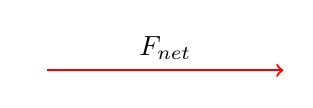
\begin{tikzpicture}
        \draw[red,thick,->]  (0,0) node[left,black] {\mymower} -- (3,0) node[above,black,pos=0.5] {$F_{\text{net}}$};
    \end{tikzpicture}
    \captionsetup{type=figure,margin=1in,font=scriptsize}
    \captionof{figure}{The net force on a lawn mower is \SI{51}{N} to the right. At what rate does the lawn mower accelerate to the right?}
\end{center}

\Solution \textit{Strategy}: Since $\vec{F}_{\text{net}}$ and $m$ are given, the acceleration can be calculated directly from Newton’s second law as stated in $\vec{F}_{\text{net}} = m \vec{a}$.

\vspace{1em}


The magnitude of the acceleration

\begin{equation*}
    a = \frac{F_{\text{net}}}{m}
\end{equation*}

Entering known values gives

\begin{equation*}
    a = \frac{\SI{51}{N}}{\SI{24}{kg}}
\end{equation*}

Substituting the units $\SI{}{kg \cdot m/s^2}$ for N yields

\begin{equation*}
    a = \frac{\SI{51}{kg \cdot m/s^2}}{\SI{24}{kg}} = \SI{2.1}{m/s^2}
\end{equation*}

\textbf{Discussion}: The direction of the acceleration is the same direction as that of the net force, which is parallel to the ground. There is no information given in this example about the individual external forces acting on the system, but we can say something about their relative magnitudes. For example, the force exerted by the person pushing the mower must be greater than the friction opposing the motion (since we know the mower moves forward), and the vertical forces must cancel if there is to be no acceleration in the vertical direction (the mower is moving only horizontally). The acceleration found is small enough to be reasonable for a person pushing a mower. Such an effort would not last too long because the person’s top speed would soon be reached.

\endsolution

\begin{example}
    \textit{What Rocket Thrust Accelerates This Sled?}\\
    Prior to space flights carrying astronauts, rocket sleds were used to test aircraft, missile equipment, and physiological effects on human subjects at high speeds. They consisted of a platform that was mounted on one or two rails and propelled by several rockets. Calculate the magnitude of force exerted by each rocket, called its thrust $\vec{T}$, for the four-rocket propulsion system shown in Figure \ref{1lc8tY}. The sled's initial acceleration is  \SI{49}{m/s2^}, the mass of the system is \SI{2100}{kg}, and the force of friction opposing the motion is known to be \SI{650}{N}.
\end{example}

\begin{center}
    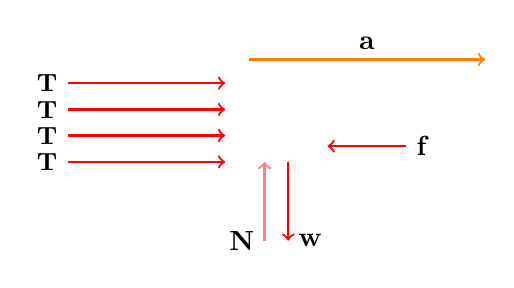
\begin{tikzpicture}
        \node[right] at (0,0) {\HUGE \mysled};
        \pgfplotsinvokeforeach{-1*0.5,-0.33*0.5,0.33*0.5,1*0.5}{
            \draw[thick,red,->] (-2,#1) node[left,black] {\small \textbf{T}} -- ++(2,0) ;
        }
        \draw[->,thick,red!50] (0.5,-1.5) node[left,black] {\textbf{N}} -- ++(0,1);
        \draw[<-,thick,red] (0.8,-1.5) node[right,black] {\textbf{w}} -- ++(0,1);
        \draw[->,thick,orange] (0.3,0.8) -- ++ (3,0) node[above,black,pos=0.5] {\textbf{a}};
        \draw[->,thick,red] (2.3,-0.3) node[right,black] {\textbf{f}} -- ++(-1,0);
    \end{tikzpicture}

    \vspace{1em}
    
    \begin{tikzpicture}
        \node at (2,2) {Free-body diagram};
        \fill[red] (0,0) circle (2pt);
        \draw[->] (-0.1,0) -- (-0.6,0) node[left] {\textbf{f}};
        \draw[->] (0,0.1) -- ++(0,1) node[above] {\textbf{N}};
        \draw[->] (0,-0.1) -- ++(0,-1) node[below] {\textbf{w}};
        \pgfplotsinvokeforeach{0.1,1.7,3.3,4.9}{
            \draw[->] (#1,0) -- ++(1.5,0) node[above,pos=0.5] {\textbf{T}};
        }
    \end{tikzpicture}
    \captionsetup{type=figure,margin=1in,font=scriptsize}
    \captionof{figure}{A sled experiences a rocket thrust that accelerates it to the right. Each rocket creates an identical thrust \textbf{T}. As in other situations where there is only horizontal acceleration, the vertical forces cancel. The ground exerts an upward force \textbf{N} on the system that is equal in magnitude and opposite in direction to its weight, \textbf{w}. The system here is the sled, its rockets, and rider, so none of the forces between these objects are considered. The arrow representing friction (\textbf{f}) is drawn larger than scale.}
    \label{1lc8tY}
\end{center}

\Solution \textit{Strategy}: Although there are forces acting vertically and horizontally, we assume the vertical forces cancel since there is no vertical acceleration. This leaves us with only horizontal forces and a simpler one-dimensional problem. Directions are indicated with plus or minus signs, with right taken as the positive direction. See the free-body diagram in the figure.

\vspace{1em}

Since acceleration, mass, and the force of friction are given, we start with Newton's second law and look for ways to find the thrust of the engines. Since we have defined the direction of the force and acceleration as acting ``to the right,'' we need to consider only the magnitudes of these quantities in the calculations. Hence we begin with

\begin{equation*}
    F_{\text{net}} = m a
\end{equation*}

where $F_{\text{net}}$ is the net force along the horizontal direction. We can see from Figure \ref{1lc8tY} that the engine thrusts add, while friction opposes the thrust. In equation form, the net external force is

\begin{equation*}
    F_{\text{net}} = 4T - f
\end{equation*}

Substituting this into Newton's second law gives

\begin{equation*}
    F_{\text{net}} = ma = 4T - f
\end{equation*}

Using a little algebra, we solve for the total thrust $4T$:

\begin{equation*}
    4T = ma + f
\end{equation*}

Substituting known values yields

\begin{equation*}
    4 T = ma + f = \left(\SI{2100}{kg}\right) \left(\SI{49}{m/s^2}\right) + \SI{650}{N}
\end{equation*}

So the total thrust is

\begin{equation*}
    4T = \SI{1.0e5}{N}
\end{equation*}

and the individual thrusts are

\begin{equation*}
    T = \frac{\SI{1.0e5}{N}}{4} = \SI{2.6e4}{N}
\end{equation*}

\textbf{Discussion}: The numbers are quite large, so the result might surprise you. Experiments such as this were performed in the early 1960s to test the limits of human endurance and the setup designed to protect human subjects in jet fighter emergency ejections. Speeds of \SI{1000}{km/h} were obtained, with accelerations of 45 $g$'s. (Recall that $g$, the acceleration due to gravity, is \SI{9.80}{m/s^2}. When we say that an acceleration is 45 $g$'s, it is  $45 \times \SI{9.80}{m/s^2}$, which is approximately  \SI{440}{m/s^2}.) While living subjects are not used any more, land speeds of \SI{10000}{km/h} have been obtained with rocket sleds. In this example, as in the preceding one, the system of interest is obvious. We will see in later examples that choosing the system of interest is crucial---and the choice is not always obvious.

\vspace{1em}

Newton's second law of motion is more than a definition; it is a relationship among acceleration, force, and mass. It can help us make predictions. Each of those physical quantities can be defined independently, so the second law tells us something basic and universal about nature. The next section introduces the third and final law of motion.

\endsolution   

\end{document}